\documentclass[a4paper,12pt]{scrartcl}  %% article, see KOMA 
\usepackage[english]{babel}
\usepackage{caption}
\captionsetup[figure]{labelfont={color=blue}}
\usepackage{color}
\usepackage[usenames,dvipsnames,svgnames,table]{xcolor}
\usepackage[backref=true,backend=bibtex,natbib=true,hyperref=true, 
style=numeric, sorting=none]{biblatex}

\addbibresource{../bibliography.bib}
\renewcommand{\labelnamepunct}{\addcolon\space} % Doppelpunkt anstatt des Punkts nach dem Autor und vor dem Titel der Arbeit
\usepackage[T1]{fontenc}
\usepackage[utf8]{inputenc}
\usepackage{lmodern}
\usepackage{ae,aecompl}
\usepackage{amsmath}
\usepackage{amsfonts}
\usepackage{amssymb}
\usepackage{psfrag}
\usepackage{authblk}
\usepackage{physics}
\usepackage{mathtools}
\usepackage{bm}
\usepackage{tikz}
\definecolor{rgray1}{gray}{0.85}
\definecolor{rgray2}{gray}{0.9}
\definecolor{rgray3}{gray}{0.95}

\renewcommand*\sectfont{\normalcolor\rmfamily\bfseries}
\renewcommand*\descfont{\rmfamily\bfseries}

%%% listings: include programming code
%\usepackage{listings}

%%% units: technical units
%\usepackage{units}
\usepackage[automark]{scrpage2}
\usepackage{ifpdf}

\ifpdf
  %%% graphicx: support for graphics
  %\usepackage[pdftex]{graphicx}
  \usepackage[pdftex=true,backref,pagebackref=false,colorlinks=true,
    bookmarks=true, bookmarksopen=false, bookmarksnumbered=false,
    pdfpagemode=None]{hyperref}
  \hypersetup{linkcolor = RoyalBlue, citecolor = RoyalBlue, urlcolor=WildStrawberry}
  \usepackage{cleveref}
  \DeclareGraphicsExtensions{.pdf}
\else
\usepackage[dvips]{graphicx}

  \DeclareGraphicsExtensions{.eps}

  \usepackage[dvips]{hyperref}
\fi

\hypersetup{
  pdftitle={Design of a broadband metamaterial absorber for the X-band}, %%
  pdfauthor={Dr. Stefan Umrath}, %%
  pdfsubject={}, %%
  pdfcreator={LaTeX with hyperref-package.}, %% 
  pdfproducer={}, %%
  pdfkeywords={} %%
}

\newcommand{\mygraphics}[3]{
  \begin{center}
    \includegraphics[width=#1, keepaspectratio=true]{#2} \\
    \textbf{#3}
  \end{center}
}
\renewcommand{\Cref}[1]{\cref{#1}\textcolor{RoyalBlue}{)}}
\newcommand{\capFref}[1]{Fig. \ref{#1}\textcolor{RoyalBlue}{)}}
\newcommand{\capEref}[1]{Eq. \textcolor{RoyalBlue}{(}\ref{#1}\textcolor{RoyalBlue}{)}}
\newcommand{\Ref}[1]{\ref{#1}\textcolor{RoyalBlue}{)}}
\newcommand{\unitv}[1]{\hat{\bm{#1}}}
\newcommand{\imag}{\mathrm{i}}
\newcommand{\euler}{\mathrm{e}}
\renewcommand{\dyad}[1]{\overset{\bm\leftrightarrow}{#1}}
\newcommand{\rd}{\mathrm{d}}
%\newcommand{\ontop}{\genfrac{\{}{\}}{0pt}{}}
\newcommand\ontop[4]{\genfrac{#1}{#2}{0pt}{}{#3}{#4}}


\title{Metamaterial Absorbers}

%%% author(s)
\author[1]{Dr. Stefan Umrath, \href{mailto:Stefan.Umrath@dlr.de}{Stefan.Umrath@dlr.de}}
\affil[1]{German Aerospace Center (DLR)}
\date{Oberpfaffenhofen \today{} \vspace{3cm}}
\bibliography{bibliography.bib}



\begin{document}

\maketitle
\begin{center}

\includegraphics[width= 0.75\linewidth]{../media/DLR_Logo_engl_schwarz.jpg}
\end{center}

\newpage
\tableofcontents 
\newpage
\section{Motivation}
Die Verwendung von elektromagnetischen Wellen hat mit der voranschreitenden 
Digitalisierung und Vernetzung stark zugenommen. Damit hat einerseits die 
Optimierung der Abstrahl-/Emfangseigenschaften von Sendern bzw. Emfängern 
an Wichtigkeit gewonnen und andererseits die Detektion von passiven, d. h. 
weder sendenden, noch empfangenden. Als Beispiele seinen die Mobilfunkkommunikation, 
autonom navigierende Fahrzeuge, oder die Luftraumüberwachung genannt, welche
sich u. a. mit der Detektion von Drohnen und feindlichen Flugzeugen beschäftigt. 
In all diesen Bereichen gibt es Anwendungen für Materialien, welche von 
Menschenhand mit einer speziellen Wirkung auf elektromagnetische Wellen
ausgestattet wurden, sog. Metamaterialien.

\section{Metamaterialien für Reflexionsdämpfung}
Überall dort, wo Reflexion von elektromagnetischen Wellen unterdrückt werden sollen
und spezielle Anforderungen an das Absorbermaterial gestellt werden, können 
Metamaterialabsorber eingesetzt werden. 
Entsprechend des Einsatzgebiets können Metamaterialabsorber ihren konventionellen
Absorbern auf Basis von magnetischen Materialien oder Schaumabsorbern in Punkto Gewicht, Dicke, Herstellungspreis überlegen sein. Je nach Anwendungszweck können Absorber mit
Wirksamkeit über einen breiten Frequenzbereich oder schmalbandig erwünscht sein. 
Um die Machbarkeit für beide Szenarien zu demonsiereren, wurden ein schmalbandiger Absorber für zwei weit verbreitete WLan-Frequnezen, sowie ein Breitbandabsorber für das militärisch relevante X-Band entwickelt, simuliert, gefertigt und vermessen.

\begin{figure}
\centering
\begin{minipage}[b]{0.4\textwidth}
\includegraphics[scale=0.3]{../media/XBandAbsorber.png}
\end{minipage}
\hspace{50pt}
\begin{minipage}[b]{0.4\textwidth}
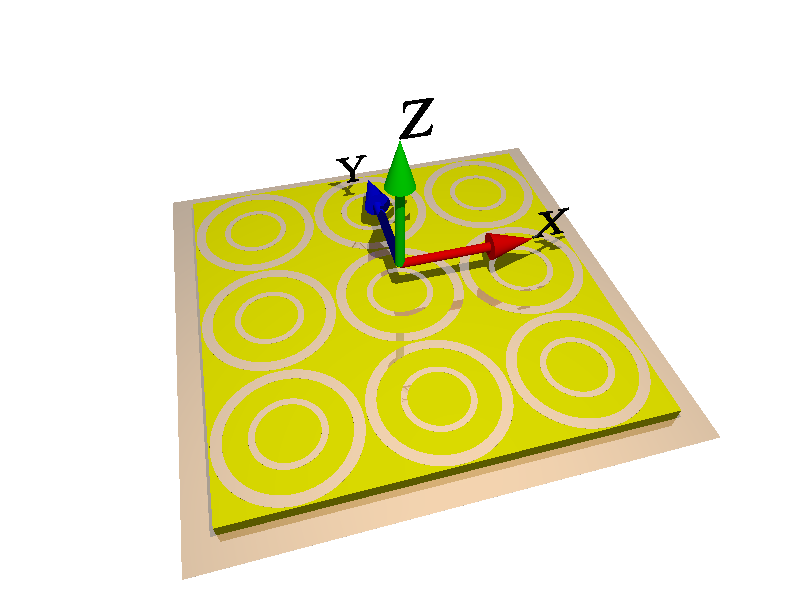
\includegraphics[scale=0.3]{../media/double_rings.png}
\end{minipage}
\end{figure}




\newpage


%%% name of the bibliography file without .bib
%%% e.g.: literatur.bib -> 

\printbibliography


\end{document}
